\documentclass[aspectratio=1610]{beamer}
\usepackage[utf8]{inputenc}
\usepackage{multicol}
\usepackage[czech]{babel}
\usepackage{amsmath}
\usepackage{csquotes}
\usepackage{bold-extra}
\usepackage{listings}
\usepackage{alltt,xcolor}

\title{Základy CSS}
\date{WBA | 7., 8. hodina}
\author[Cajthaml]{Matěj Cajthaml}

\usetheme{material}

\usePrimaryCustom

\begin{document}

\begin{frame}
\titlepage
\end{frame}

\begin{frame}{Obsah prezentace}
    \begin{cardTiny}
        \begin{minipage}{\textwidth}
            \vspace{1ex}
            \tableofcontents
        \end{minipage}
    \end{cardTiny}
\end{frame}

\section{Opakování HTML}


\section{Co je to CSS}

\begin{frameImg}[width]{img/cssrender.png}
    \vspace*{60mm}
    \begin{cardTiny}
        \vspace*{\fill}
        \begin{center}
            \textbf{CSS}
        \end{center}
    \end{cardTiny}
\end{frameImg}

\begin{frame}{CSS}
    \begin{cardTiny}
        \begin{flushleft}
            = \textbf{Cascading Style Sheets}.

            Definice stylů stránky, které jsou nezávislé na HTML.

            Způsob zobrazení (designu) prvků na stránce.

            \vspace{2ex}
            Barva a velikost písma, zarovnání, rámečky, odsazení...
        \end{flushleft}
    \end{cardTiny}
\end{frame}

\begin{frame}{Výhody a nevýhody CSS}
    \begin{multicols}{2}
        \centering

        \begin{cardTiny}
            \begin{center}
                \textbf{VÝHODY}
            \end{center}

            \begin{flushleft}
            Konkrétní prvky, třídy a identifikátory.

            Rychlejší načítání - méně kódu.

            Vše se dá jednoduše upravovat na jednom místě.
            \end{flushleft}
        \end{cardTiny}

        \begin{cardTiny}
            \begin{center}
                \textbf{NEVÝHODY}
            \end{center}
        
            Problémy s prohlížeči.

            Nevyužité styly se přesto musí načíst.
        \end{cardTiny}
    \end{multicols}
\end{frame}

\begin{frame}{Soubory CSS}
    \begin{cardTiny}
        Přípona \texttt{.css}.

        Bez diakritiky, mezer, malými písmeny.
    \end{cardTiny}
\end{frame}



\section{Jak se CSS zapisuje}

\begin{frame}{Syntaxe}
    \begin{cardTiny}
        \begin{flushleft}
            \textcolor{red}{Selektor} - výběr prvku

            \textcolor{blue}{Vlastnost} - vlastnost, které definujeme hodnotu

            \textcolor{orange}{Hodnota} - samotná hodnota vlastnosti
        \end{flushleft}
    \end{cardTiny}

    \begin{cardTiny}
        \begin{alltt}
            \textcolor{red}{selektor} \string{\\
            \textcolor{blue}{vlastnost}: \textcolor{orange}{hodnota};\\
            \string}
        \end{alltt}
    \end{cardTiny}
\end{frame}

\begin{frame}{Implementace stylů}
    \begin{multicols}{2}
        \centering

        \begin{cardTiny}
            \begin{center}
                \textbf{INLINE}
            \end{center}

            \begin{flushleft}
                Použití atributu style v tagu.

                Platí pouze pro daný tag. 

                CSS poté ztrácí smysl, nepřehlednost.
            \end{flushleft}
        \end{cardTiny}
        \begin{cardTiny}
            \begin{center}
                \textbf{EMBED}
            \end{center}
        
            \begin{flushleft}
                Umístění přímo na stránce v hlavičce (tagu head).

                Styly se aplikují na celou stránku.
            \end{flushleft}
        \end{cardTiny}
        \begin{cardTiny}
            \begin{center}
                \textbf{EXTERNAL}
            \end{center}
        
            \begin{flushleft}
                Samostatný soubor s CSS.

                Prováže se s dokumentem pomocí tagu link.
            \end{flushleft}
        \end{cardTiny}
        \begin{cardTiny}
            \begin{center}
                \textbf{IMPORT}
            \end{center}
        
            \begin{flushleft}
                Vložení CSS souboru do definice CSS.
            \end{flushleft}
        \end{cardTiny}
    \end{multicols}
\end{frame}

\begin{frame}{Jednoduché selektory 1}
    \begin{multicols}{2}
        \centering

        \begin{cardTiny}
            \begin{center}
                \textbf{TAG}
            \end{center}

            \begin{flushleft}
                \begin{alltt}
                    \textcolor{red}{b} \string{\\
                        \textcolor{blue}{color}: \textcolor{orange}{blue};\\
                    \string}
                \end{alltt}
                \begin{alltt}
                    <p>text <b>tlusty</b> ne</p>
                \end{alltt}
            \end{flushleft}
        \end{cardTiny}
        \begin{cardTiny}
            \begin{center}
                \textbf{VŠE}
            \end{center}

            \begin{flushleft}
                \begin{alltt}
                    \textbf{\textcolor{red}{*}} \string{\\
                        \textcolor{blue}{color}: \textcolor{orange}{purple};\\
                    \string}
                \end{alltt}

                \begin{alltt}
                    <p>text <b>tlusty</b> ano</p>
                \end{alltt}
            \end{flushleft}
        \end{cardTiny}
    \end{multicols}
\end{frame}

\begin{frame}{Jednoduché selektory 2}
    \begin{multicols}{2}
        \centering

        \begin{cardTiny}
            \begin{center}
                \textbf{TŘÍDA}
            \end{center}

            \begin{flushleft}
                \begin{alltt}
                    \textbf{\textcolor{red}{.moje-trida}} \string{\\
                        \textcolor{blue}{color}: \textcolor{orange}{cyan};\\
                    \string}
                \end{alltt}
                \begin{alltt}
                    <p class=''moje-trida''>text</p>
                \end{alltt}
            \end{flushleft}
        \end{cardTiny}
        \begin{cardTiny}
            \begin{center}
                \textbf{IDENTIFIKATOR}
            \end{center}

            \begin{flushleft}
                \begin{alltt}
                    \textbf{\textcolor{red}{\#muj}} \string{\\
                        \textcolor{blue}{color}: \textcolor{orange}{lime};\\
                    \string}
                \end{alltt}
                \begin{alltt}
                    <p id=''muj''>Kocour</p>
                \end{alltt}
            \end{flushleft}
        \end{cardTiny}
    \end{multicols}
\end{frame}

\begin{frame}{Ukázka syntaxe}
    \begin{center}
        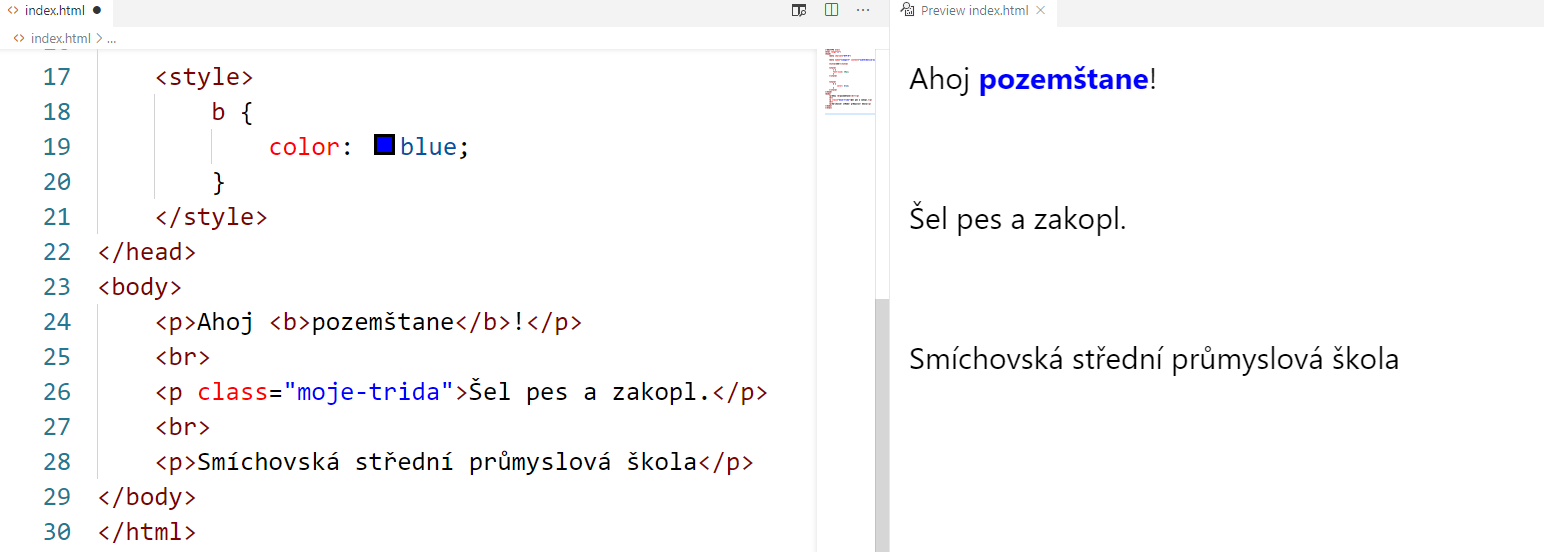
\includegraphics[width=\textwidth]{img/html-7-8-1.png}
    \end{center}
\end{frame}

\begin{frame}{Seskupování}
    \begin{cardTiny}
        \begin{flushleft}
            \begin{alltt}
                \textbf{\textcolor{red}{b}, \textcolor{red}{.moje-trida}} \string{\\
                    \textcolor{blue}{color}: \textcolor{orange}{blue};\\
                \string}
            \end{alltt}
            \begin{alltt}
                <p>Ahoj <b>pozemštane</b>!</p>

                <br>
                
                <p class=''moje-trida''>Šel pes a zakopl.</p>
                
                <br>
                
                <p>Smíchovská střední průmyslová škola</p>
            \end{alltt}
        \end{flushleft}
    \end{cardTiny}
    \begin{cardTiny}
        \begin{center}
            \textbf{Co bude modré?}
        \end{center}
    \end{cardTiny}
\end{frame}

\begin{frame}{Modrá je dobrá!}
    \begin{center}
        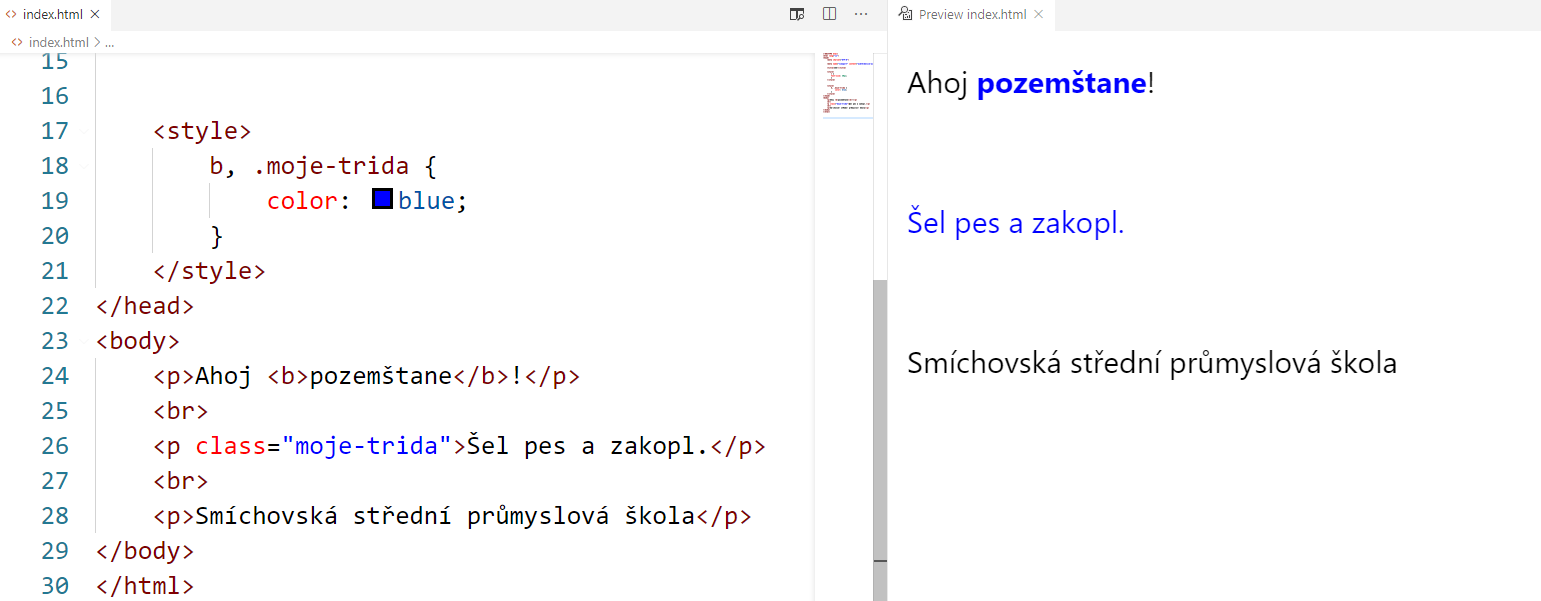
\includegraphics[width=\textwidth]{img/html-7-8-2.png}
    \end{center}
\end{frame}

\begin{frame}{Dedičnost}
    \begin{cardTiny}
        Vlastnosti se z rodiče předávají všem dětem.

        Předávají se i před další děti, pokud je jejich rodič nepřepíše.
    \end{cardTiny}
\end{frame}

\begin{frame}{Komentáře v CSS}
    \begin{cardTiny}
        \begin{center}
        \texttt{/*} komentář \texttt{*/}
        \end{center}
    \end{cardTiny}
\end{frame}


\section{Text v HTML}
\begin{frame}{Prostý text}
    \begin{cardTiny}
        \begin{flushleft}
            Zápis: \begin{alltt}\textbf{$<$\textcolor{red}{p}$>$}Obyčejný text\textbf{$<$/\textcolor{red}{p}$>$}\end{alltt}
        \end{flushleft}
    \end{cardTiny}
\end{frame}

\begin{frame}{Nadpisy}
    \begin{cardTiny}
        \begin{flushleft}
            Zápis: \begin{alltt}\textbf{$<$\textcolor{red}{h}\textcolor{red}{(cislo)}$>$}Nadpis\textbf{$<$/\textcolor{red}{h}\textcolor{red}{(cislo)}$>$}\end{alltt}
        
            Číslo - úroveň nadpisu. Od 1 (největší) do 6 (nejmenší).

            Hierarchie

            První úroveň - jen jednou.
        \end{flushleft}
    \end{cardTiny}
\end{frame}

\begin{frame}{Nadpisy špatně!}
    \begin{center}
        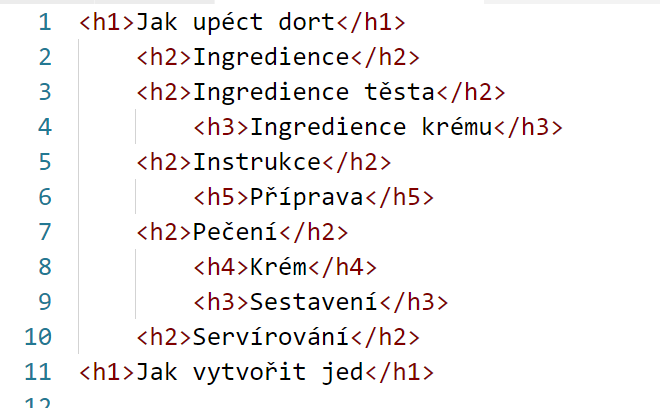
\includegraphics[width=0.8\textwidth]{img/html-cake-bad.png}
    \end{center}
\end{frame}

\begin{frame}{Nadpisy správně!}
    \begin{center}
        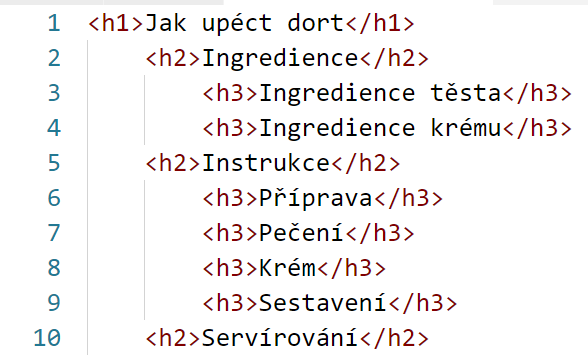
\includegraphics[width=0.8\textwidth]{img/html-cake.png}
    \end{center}
\end{frame}

\begin{frame}{Formátování textu - zalamování řádku}
    \begin{cardTiny}
        \begin{flushleft}
            \textit{line BReak} = Nová řádka

            Zápis: \begin{alltt}\textbf{$<$\textcolor{red}{br}$ />$}\end{alltt}
        \end{flushleft}
    \end{cardTiny}
\end{frame}

\begin{frame}{Formátování textu - vodorovná čára}
    \begin{cardTiny}
        \begin{flushleft}
            \textit{Horizontal Rule} = Čára k oddělení obsahu 

            Zápis: \begin{alltt}\textbf{$<$\textcolor{red}{hr}$ />$}\end{alltt}
        \end{flushleft}
    \end{cardTiny}
\end{frame}

\begin{frame}{Formátování textu - tlusté písmo}
    \begin{cardTiny}
        \begin{flushleft}
            Zápis: \begin{alltt}\textbf{$<$\textcolor{red}{b}$>$}Tlustý text\textbf{$<$/\textcolor{red}{b}$>$}\end{alltt}
        \end{flushleft}
    \end{cardTiny}
\end{frame}

\begin{frame}{Formátování textu - kurzíva}
    \begin{cardTiny}
        \begin{flushleft}
            Zápis: \begin{alltt}\textbf{$<$\textcolor{red}{i}$>$}Text kurzívou\textbf{$<$/\textcolor{red}{i}$>$}\end{alltt}
        \end{flushleft}
    \end{cardTiny}
\end{frame}

\begin{frame}{Formátování textu - indexy}
    \begin{cardTiny}
        \begin{flushleft}
            Zápis: \begin{alltt}\textbf{$<$\textcolor{red}{sup}$>$}Horní index\textbf{$<$/\textcolor{red}{sup}$>$}\end{alltt}
        \end{flushleft}
    \end{cardTiny}
    \begin{cardTiny}
        \begin{flushleft}
            Zápis: \begin{alltt}\textbf{$<$\textcolor{red}{sub}$>$}Dolní index\textbf{$<$/\textcolor{red}{sub}$>$}\end{alltt}
        \end{flushleft}
    \end{cardTiny}
\end{frame}

\begin{frame}{Formátování textu - přeškrtnutí}
    \begin{cardTiny}
        \begin{flushleft}
            Zápis: \begin{alltt}\textbf{$<$\textcolor{red}{s}$>$}Přeškrtnutý text\textbf{$<$/\textcolor{red}{s}$>$}\end{alltt}
        \end{flushleft}
    \end{cardTiny}
\end{frame}



\section{CSS hodnoty}

\begin{frame}{CSS barvy - název}
    \begin{cardTiny}
        \begin{flushleft} 
            \begin{alltt}
                \textcolor{red}{.barevnak} \string{\\
                    \textcolor{blue}{color}: \textcolor{orange}{blue};\\
                \string}
            \end{alltt}

            \vspace{2ex}

            \href{https://www.w3schools.com/cssref/css_colors.asp}{ODKAZ - předefinované barvy v CSS}
        \end{flushleft}
    \end{cardTiny}
\end{frame}

\begin{frame}{CSS barvy - RGB(A)}
    \begin{cardTiny}
        \begin{flushleft} 
            Skládá se ze tří barev - červená (Red), zelená (Green), modrá (Blue).

            Nastavitelná průhlednost od 0 do 1.

            Maximum - bílá barva.

            \begin{alltt}
                \textcolor{red}{.barevnak} \string{\\
                    \textcolor{blue}{color}: \textcolor{orange}{rgb(255, 0, 0)};\\
                \string}
            \end{alltt}

            \begin{alltt}
                \textcolor{red}{.barevnak} \string{\\
                    \textcolor{blue}{color}: \textcolor{orange}{rgb(255, 255, 0, 0.5)};\\
                \string}
            \end{alltt}
        \end{flushleft}
    \end{cardTiny}
\end{frame}

\begin{frame}{CSS barvy - HEX}
    \begin{cardTiny}
        \begin{flushleft}
            Podobné jako u RGB.

            Barvy se udávají ve třech částech - v šestnáckové soustavě.

            Čtyři části - průhlednost.

            255 = FF, 0 = 00, 120 = 78

            \begin{alltt}
                \textcolor{red}{.barevnak} \string{\\
                    \textcolor{blue}{color}: \textcolor{orange}{\#FF0000};\\
                \string}
            \end{alltt}

            \begin{alltt}
                \textcolor{red}{.barevnak} \string{\\
                    \textcolor{blue}{color}: \textcolor{orange}{\#FF7878F0};\\
                \string}
            \end{alltt}
        \end{flushleft}
    \end{cardTiny}
\end{frame}

\begin{frame}{CSS jednotky}
    \begin{cardTiny}
        Relativní vs. absolutní jednotka

        \begin{center}
            \begin{tabular}{ |c|c|c| } 
                \hline
                px & jeden pixel na obrazovce & 100px \\ 
                cm & centimetr = 37.8px & 5cm \\ 
                em & výška řádku & 1.5em \\ 
                \% & šírka daného rodiče & 55\% \\ 
                vh & procento dostupné výšky prohlížeče & 100vh \\ 
                \hline
            \end{tabular}
        \end{center}
    \end{cardTiny}

    \begin{cardTiny}
        \begin{alltt}
            \textcolor{red}{.dulezite} \string{\\
                \textcolor{blue}{font-size}: \textcolor{orange}{5em};\\
            \string}
        \end{alltt}
    \end{cardTiny}
\end{frame}



\section{Základní CSS vlastnosti}

\begin{frame}{CSS vlastnosti - background-color}
    \begin{cardTiny}
        Nastavení barvy pozadí.

        \begin{alltt}
            \textcolor{red}{.barva} \string{\\
                \textcolor{blue}{background-color}: \textcolor{orange}{white};\\
            \string}
        \end{alltt}
    \end{cardTiny}
\end{frame}

\begin{frame}{CSS vlastnosti - text-align}
    \begin{cardTiny}
        Zarovnání textu.

        Možné hodnoty: left, right, center, justify

        \begin{alltt}
            \textcolor{red}{.prostredek} \string{\\
                \textcolor{blue}{text-align}: \textcolor{orange}{center};\\
            \string}
        \end{alltt}
    \end{cardTiny}
\end{frame}

\begin{frame}{CSS vlastnosti - font-family}
    \begin{cardTiny}
        Určení fontu písma.

        Písmo na PC / importováno.

        Priorita fontů.

        \begin{alltt}
            \textcolor{red}{.special} \string{\\
                \textcolor{blue}{font-family}: \textcolor{orange}{"Times New Roman", "Roboto", serif};\\
            \string}
        \end{alltt}
    \end{cardTiny}
\end{frame}

\begin{frame}{CSS vlastnosti - font-size}
    \begin{cardTiny}
        Nastavení velikosti písma.

        \begin{alltt}
            \textcolor{red}{.special} \string{\\
                \textcolor{blue}{font-size}: \textcolor{orange}{40px};\\
            \string}
        \end{alltt}
    \end{cardTiny}
\end{frame}

\begin{frame}{CSS vlastnosti - font-style}
    \begin{cardTiny}
        Nastavení typu písma.

        Možné hodnoty: normal, italic.

        \begin{alltt}
            \textcolor{red}{.special} \string{\\
                \textcolor{blue}{font-style}: \textcolor{orange}{italic};\\
            \string}
        \end{alltt}
    \end{cardTiny}
\end{frame}

\begin{frame}{CSS vlastnosti - font-weight}
    \begin{cardTiny}
        Nastavení tloušťky písma.

        Možné hodnoty: bold, 100 - 900, bolder, lighter, ...

        \begin{alltt}
            \textcolor{red}{.special} \string{\\
                \textcolor{blue}{font-weight}: \textcolor{orange}{bold};\\
            \string}
        \end{alltt}
    \end{cardTiny}
\end{frame}

\begin{frame}{CSS vlastnosti - text-decoration}
    \begin{cardTiny}
        Nastavení speciálního formátování textu.

        Možné hodnoty: overline, line-through, underline

        Možnosti kombinace

        \begin{alltt}
            \textcolor{red}{.special} \string{\\
                \textcolor{blue}{text-decoration}: \textcolor{orange}{overline underline};\\
            \string}
        \end{alltt}
    \end{cardTiny}
\end{frame}


\section{Shrnutí}

\begin{frame}
    \begin{center}
        
\includegraphics[width=\textwidth]{img/html-7-8-ukol.png}
    \end{center}
\end{frame}

\end{document}